\documentclass[11pt,a4paper]{report}
\usepackage[textwidth=37em,vmargin=30mm]{geometry}
\usepackage{calc,xunicode,amsmath,amssymb,paralist,enumitem,tabu,booktabs,datetime2,xeCJK,xeCJKfntef,listings}
\usepackage{tocloft,fancyhdr,tcolorbox,xcolor,graphicx,eso-pic,xltxtra,xelatexemoji}

\newcommand{\envyear}[0]{2025}
\newcommand{\envdatestr}[0]{2025-05-11}
\newcommand{\envfinaldir}[0]{webdb/2025/20250511/final}

\usepackage[hidelinks]{hyperref}
\hypersetup{
    colorlinks=false,
    pdfpagemode=FullScreen,
    pdftitle={Web Digest - \envdatestr}
}

\setlength{\cftbeforechapskip}{10pt}
\renewcommand{\cftchapfont}{\rmfamily\bfseries\large\raggedright}
\setlength{\cftbeforesecskip}{2pt}
\renewcommand{\cftsecfont}{\sffamily\small\raggedright}

\setdefaultleftmargin{2em}{2em}{1em}{1em}{1em}{1em}

\usepackage{xeCJK,xeCJKfntef}
\xeCJKsetup{PunctStyle=plain,RubberPunctSkip=false,CJKglue=\strut\hskip 0pt plus 0.1em minus 0.05em,CJKecglue=\strut\hskip 0.22em plus 0.2em}
\XeTeXlinebreaklocale "zh"
\XeTeXlinebreakskip = 0pt


\setmainfont{Brygada 1918}
\setromanfont{Brygada 1918}
\setsansfont{IBM Plex Sans}
\setmonofont{JetBrains Mono NL}
\setCJKmainfont{Noto Serif CJK SC}
\setCJKromanfont{Noto Serif CJK SC}
\setCJKsansfont{Noto Sans CJK SC}
\setCJKmonofont{Noto Sans CJK SC}

\setlength{\parindent}{0pt}
\setlength{\parskip}{8pt}
\linespread{1.15}

\lstset{
	basicstyle=\ttfamily\footnotesize,
	numbersep=5pt,
	backgroundcolor=\color{black!5},
	showspaces=false,
	showstringspaces=false,
	showtabs=false,
	tabsize=2,
	captionpos=b,
	breaklines=true,
	breakatwhitespace=true,
	breakautoindent=true,
	linewidth=\textwidth
}






\newcommand{\coverpic}[2]{
    % argv: itemurl, authorname
    Cover photo by #2~~(\href{#1}{#1})
}
\newcommand{\makeheader}[0]{
    \begin{titlepage}
        % \newgeometry{hmargin=15mm,tmargin=21mm,bmargin=12mm}
        \begin{center}
            
            \rmfamily\scshape
            \fontspec{BaskervilleF}
            \fontspec{Old Standard}
            \fontsize{59pt}{70pt}\selectfont
            WEB\hfill DIGEST
            
            \vfill
            % \vskip 30pt
            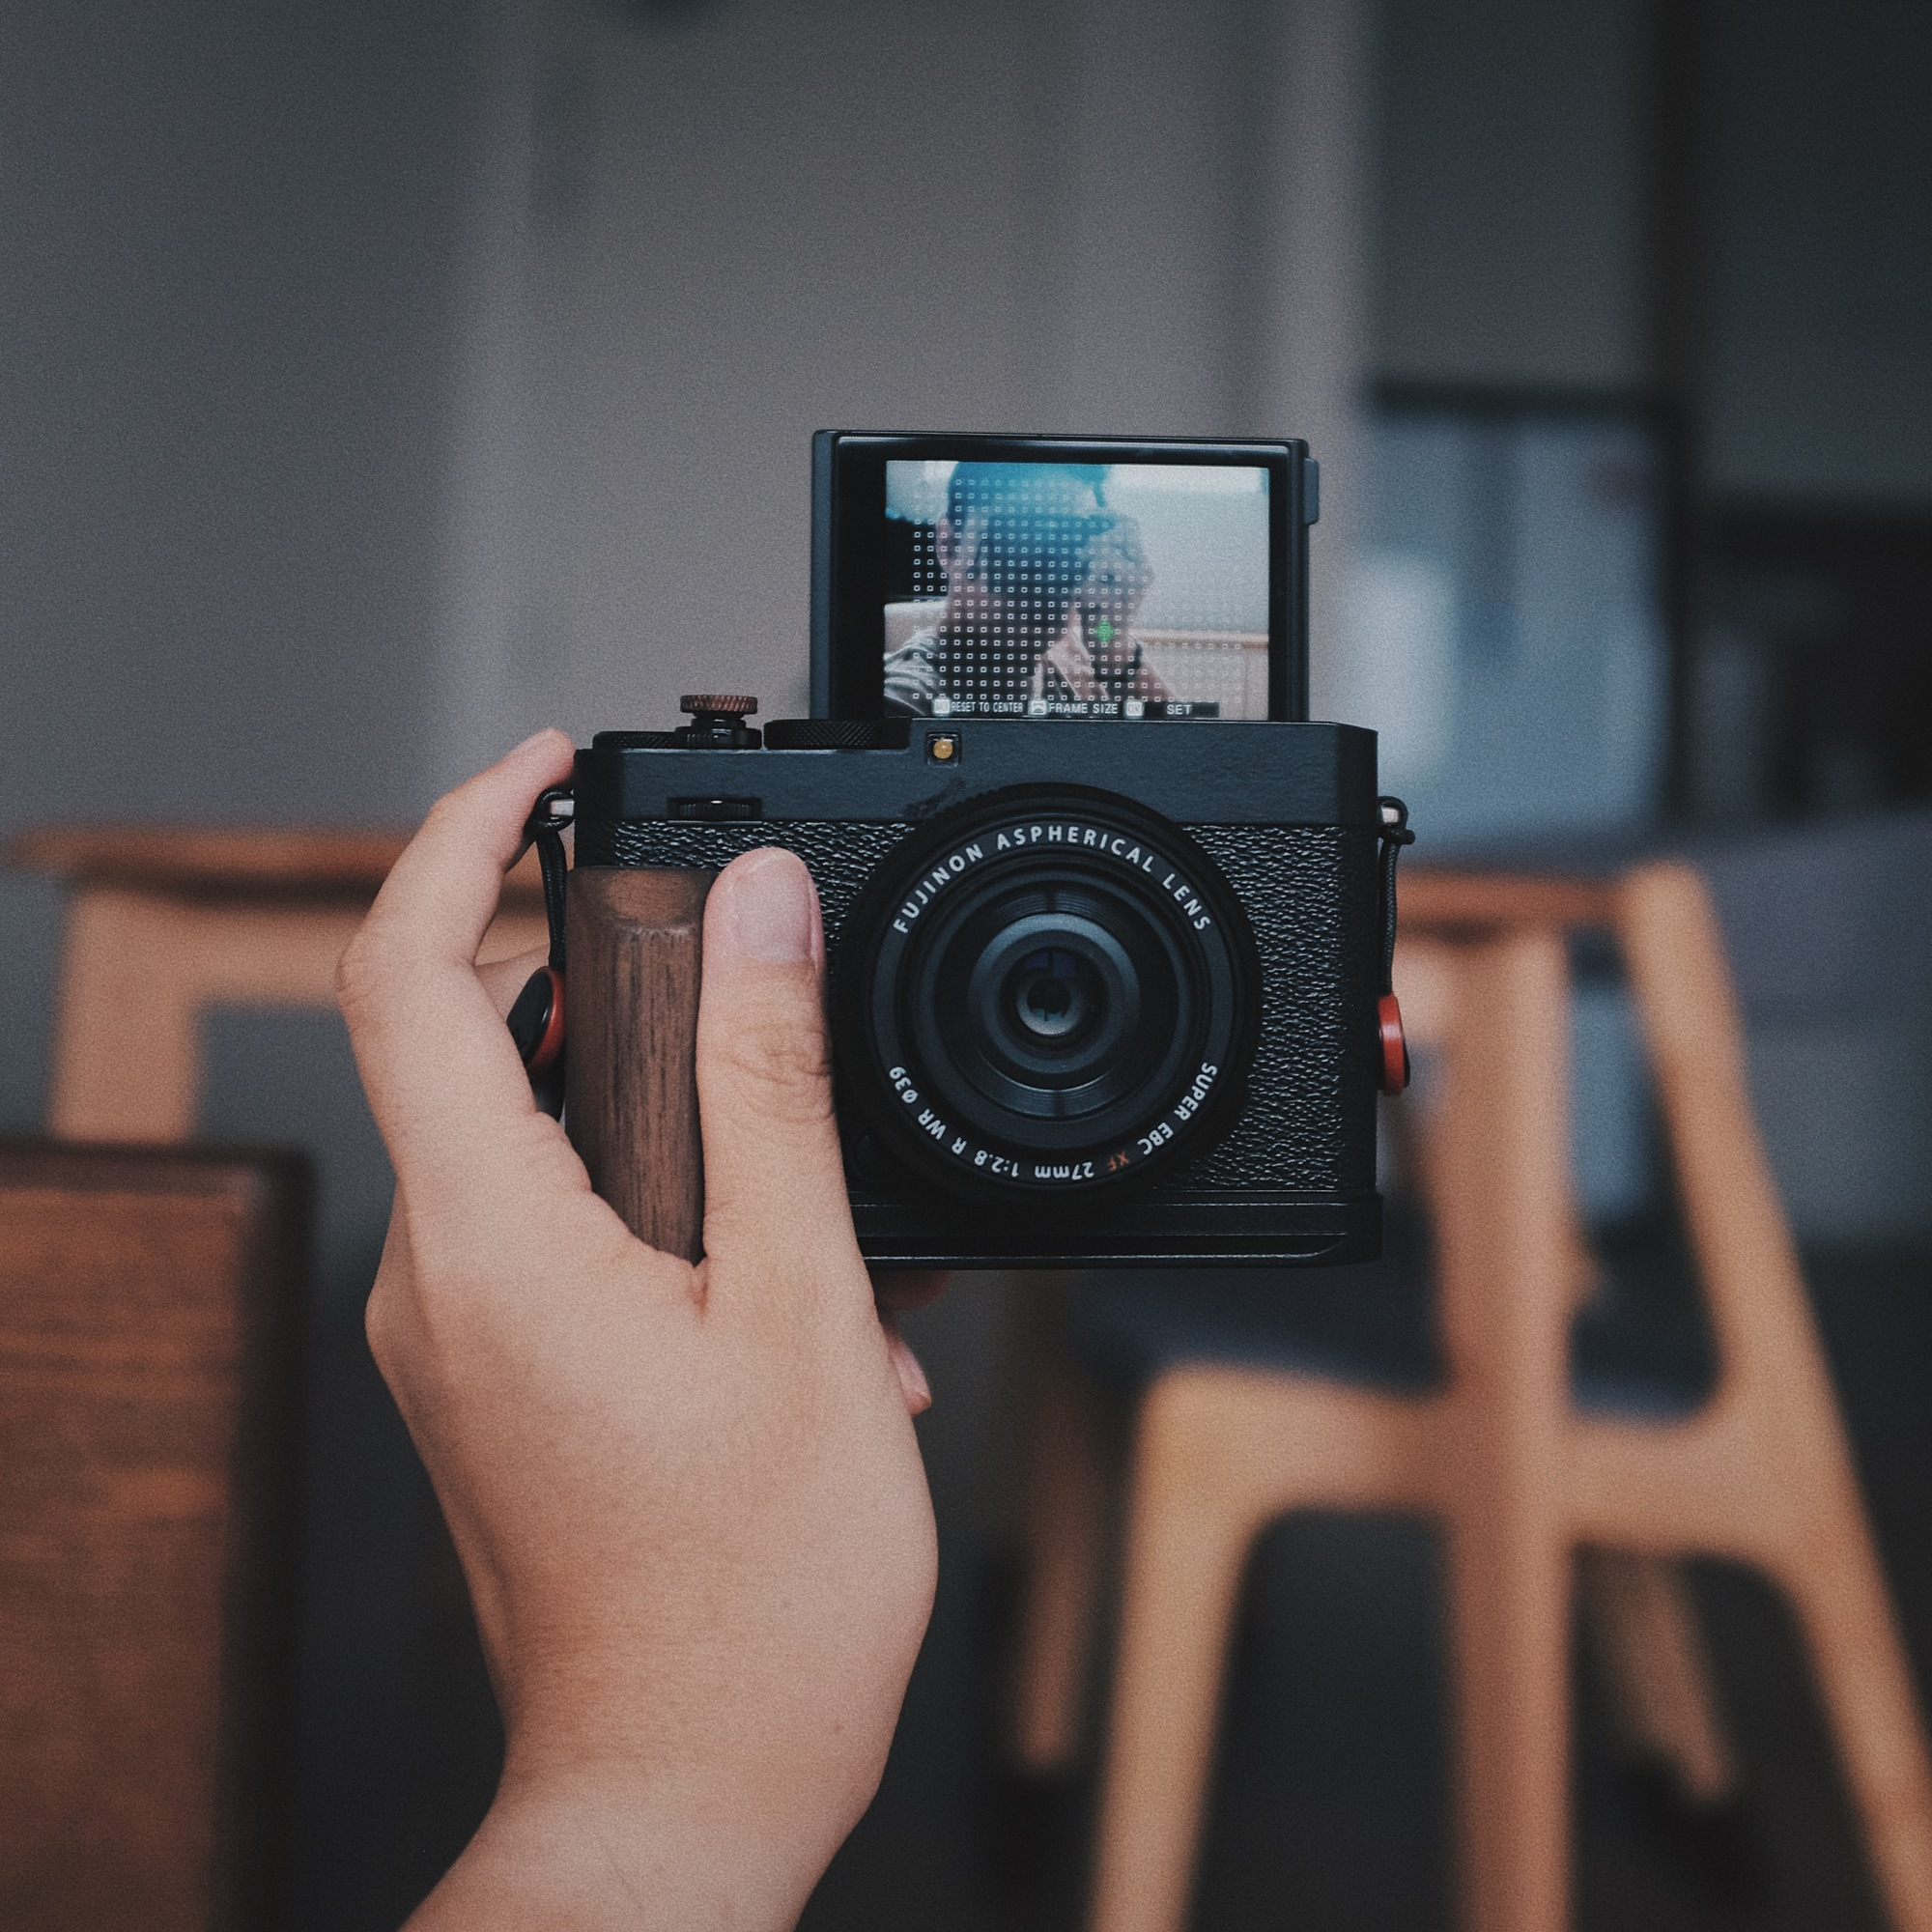
\includegraphics[width=\linewidth]{\envfinaldir/coverpic-prod.jpg}\par
            % \vskip 30pt
            \vfill

            \normalsize\rmfamily\scshape
            \copyright{} The Web Digest Project \hfill\large \envdatestr
        \end{center}
    \end{titlepage}
    % \restoregeometry
}
\newcommand{\simplehref}[1]{%
    \textcolor{blue!80!green}{\href{#1}{#1}}%
}
\renewcommand{\contentsname}{\center\Huge\sffamily\bfseries Contents\par\vskip 20pt}
\newcounter{ipartcounter}
\setcounter{ipartcounter}{0}
\newcommand{\ipart}[1]{
    % \vskip 20pt
    \clearpage
    \stepcounter{ipartcounter}
    \phantomsection
    \addcontentsline{toc}{chapter}{#1}
    % \begin{center}
    %     \Huge
    %     \sffamily\bfseries
    %     #1
    % \end{center}
    % \vskip 20pt plus 7pt
}
\newcounter{ichaptercounter}
\setcounter{ichaptercounter}{0}
\newcommand{\ichapter}[1]{
    % \vskip 20pt
    \clearpage
    \stepcounter{ichaptercounter}
    \phantomsection
    \addcontentsline{toc}{section}{\numberline{\arabic{ichaptercounter}}#1}
    \begin{center}
        \Huge
        \sffamily\bfseries
        #1
    \end{center}
    \vskip 20pt plus 7pt
}
\newcommand{\entrytitlefont}[1]{\subsection*{\raggedright\Large\sffamily\bfseries#1}}
\newcommand{\entryitemGeneric}[2]{
    % argv: title, url
    \parbox{\linewidth}{
        \entrytitlefont{#1}\par\vskip 5pt
        \footnotesize\ttfamily\mdseries
        \simplehref{#2}
    }\vskip 11pt plus 11pt minus 1pt
}
\newcommand{\entryitemGithub}[3]{
    % argv: title, url, desc
    \parbox{\linewidth}{
        \entrytitlefont{#1}\par\vskip 5pt
        \footnotesize\ttfamily\mdseries
        \simplehref{#2}\par\vskip 5pt
        \small\rmfamily\mdseries#3
    }\vskip 11pt plus 11pt minus 1pt
}
\newcommand{\entryitemAp}[3]{
    % argv: title, url, desc
    \parbox{\linewidth}{
        \entrytitlefont{#1}\par\vskip 5pt
        \footnotesize\ttfamily\mdseries
        \simplehref{#2}\par\vskip 5pt
        \small\rmfamily\mdseries#3
    }\vskip 11pt plus 11pt minus 1pt
}
\newcommand{\entryitemHackernews}[3]{
    % argv: title, hnurl, rawurl
    % \parbox{\linewidth}{
    %     \entrytitlefont{#1}\par\vskip 5pt
    %     \footnotesize\ttfamily\mdseries
    %     \simplehref{#3}\par
    %     \textcolor{black!50}{\href{#2}{#2}}
    % }\vskip 11pt plus 11pt minus 1pt
    \begin{minipage}{\linewidth}
            \entrytitlefont{#1}\par\vskip 5pt
            \footnotesize\ttfamily\mdseries
            \simplehref{#3}\par
            \textcolor{black!50}{\href{#2}{#2}}
    \end{minipage}\par\vskip 11pt plus 11pt minus 1pt
}







\begin{document}

\makeheader

\tableofcontents\clearpage




\ipart{Developers}
\ichapter{Hacker News}
\entryitemTwoLinks{For \$595, you get what nobody else can give you for twice the price (1982) [pdf]}{https://news.ycombinator.com/item?id=43947630}{https://s3data.computerhistory.org/brochures/commodore.commodore64.1982.102646264.pdf}

\entryitemTwoLinks{Reverse engineering the 386 processor's prefetch queue circuitry}{https://news.ycombinator.com/item?id=43946824}{http://www.righto.com/2025/05/386-prefetch-circuitry-reverse-engineered.html}

\entryitemTwoLinks{Sam Altman Wants Your Eyeball}{https://news.ycombinator.com/item?id=43946766}{https://www.privacyguides.org/articles/2025/05/10/sam-altman-wants-your-eyeball/}

\entryitemTwoLinks{'We Currently Have No Container Ships,' Seattle Port Says}{https://news.ycombinator.com/item?id=43946601}{https://www.newsweek.com/seattle-port-says-no-container-ships-tariffs-2069464}

\entryitemTwoLinks{'It cannot provide nuance': UK experts warn AI therapy chatbots are not safe}{https://news.ycombinator.com/item?id=43946498}{https://www.theguardian.com/technology/2025/may/07/experts-warn-therapy-ai-chatbots-are-not-safe-to-use}

\entryitemTwoLinks{A Critical Look at MCP}{https://news.ycombinator.com/item?id=43945993}{https://raz.sh/blog/2025-05-02\_a\_critical\_look\_at\_mcp}

\entryitemTwoLinks{US vs. Google amicus curiae brief of Y Combinator in support of plaintiffs [pdf]}{https://news.ycombinator.com/item?id=43945820}{https://storage.courtlistener.com/recap/gov.uscourts.dcd.223205/gov.uscourts.dcd.223205.1300.1.pdf}

\entryitemTwoLinks{The cult of doing business}{https://news.ycombinator.com/item?id=43945162}{https://www.commonwealmagazine.org/calvert-work-entrepreneur-ethic-baker-review-job}

\entryitemTwoLinks{LTXVideo 13B AI video generation}{https://news.ycombinator.com/item?id=43944974}{https://ltxv.video/}

\entryitemTwoLinks{Embracer Games Archive is preserving 75000 video games and needs contributions}{https://news.ycombinator.com/item?id=43944789}{https://embracergamesarchive.com/}

\entryitemTwoLinks{The Deathbed Fallacy (2018)}{https://news.ycombinator.com/item?id=43944467}{https://www.hjorthjort.xyz/2018/02/21/the-deathbed-fallacy.html}

\entryitemTwoLinks{Slow software for a burning world}{https://news.ycombinator.com/item?id=43943652}{https://bonfirenetworks.org/posts/slow\_software\_for\_a\_burning\_world/}

\entryitemTwoLinks{Europe launches program to lure scientists away from the US}{https://news.ycombinator.com/item?id=43943583}{https://es.wired.com/articulos/europa-lanza-iniciativa-para-atraer-talento-cientifico-tras-recortes-en-ee-uu}

\entryitemTwoLinks{Gmail to SQLite}{https://news.ycombinator.com/item?id=43943236}{https://github.com/marcboeker/gmail-to-sqlite}

\entryitemTwoLinks{Vision Now Available in Llama.cpp}{https://news.ycombinator.com/item?id=43943047}{https://github.com/ggml-org/llama.cpp/blob/master/docs/multimodal.md}

\entryitemTwoLinks{A simple 16x16 dot animation from simple math rules}{https://news.ycombinator.com/item?id=43942881}{https://tixy.land}

\entryitemTwoLinks{Brandon's Semiconductor Simulator}{https://news.ycombinator.com/item?id=43942279}{https://brandonli.net/semisim/}

\entryitemTwoLinks{WebGL Water (2010)}{https://news.ycombinator.com/item?id=43942149}{https://madebyevan.com/webgl-water/}

\entryitemTwoLinks{Fleurs du Mal}{https://news.ycombinator.com/item?id=43941598}{https://fleursdumal.org}

\entryitemTwoLinks{Era of U.S. dollar may be winding down}{https://news.ycombinator.com/item?id=43940865}{https://news.harvard.edu/gazette/story/2025/05/era-of-u-s-dollar-may-be-winding-down/}\ichapter{Phoronix}
\entryitemGeneric{\hskip 0pt{}Bcachefs, Btrfs, EXT4, F2FS \& XFS File-System Performance On Linux 6.15}{https://www.phoronix.com/review/linux-615-filesystems}

\entryitemGeneric{\hskip 0pt{}KDE Plasma Will Now Make Sure Your System Doesn't Suspend When Transferring Files}{https://www.phoronix.com/news/KDE-No-Suspend-On-Transfer-File}

\entryitemGeneric{\hskip 0pt{}Linux Lands Fix For Some TLB Flushes Being Inadvertently Skipped}{https://www.phoronix.com/news/Linux-Fixes-TLB-Flush-Skipping}

\entryitemGeneric{\hskip 0pt{}Servo Browser Engine Now Rendering Gmail \& Google Chat, Decides Against AI Contributions}{https://www.phoronix.com/news/Servo-Gmail-Now-Works}

\entryitemGeneric{\hskip 0pt{}FreeBSD 14.3 Beta 2 Brings WiFi Fixes, Reproducible ARM64 Kernel Binary Build}{https://www.phoronix.com/news/FreeBSD-14.3-Beta-2}

\entryitemGeneric{\hskip 0pt{}GNOME Showtime Accepted As Video Player App For GNOME 49}{https://www.phoronix.com/news/GNOME-49-Video-Player-Showtime}

\entryitemGeneric{\hskip 0pt{}Samsung Odyssey OLED G8 G81SF 4K UHD HDR Monitor}{https://www.phoronix.com/review/samsung-g8-g81sf}

\entryitemGeneric{\hskip 0pt{}RADV Vulkan Driver Lands BFloat16 Support In Mesa 25.2}{https://www.phoronix.com/news/RADV-Shader-BFloat16}

\entryitemGeneric{\hskip 0pt{}DeepComputing's DC-ROMA RISC-V Mainboard II For Framework Laptop Launches For \$349}{https://www.phoronix.com/news/DC-ROMA-RISC-V-Framework-Launch}\ichapter{Dribbble}
\entryitemGeneric{\hskip 0pt{}Logo Roundup > Elegant Vibe}{https://dribbble.com/shots/26000783-Logo-Roundup-Elegant-Vibe}

\entryitemGeneric{\hskip 0pt{}CTRL the Chaos // Dashboard}{https://dribbble.com/shots/25997365-CTRL-the-Chaos-Dashboard}

\entryitemGeneric{\hskip 0pt{}JOUI-yoga for kids}{https://dribbble.com/shots/25997787-JOUI-yoga-for-kids}

\entryitemGeneric{\hskip 0pt{}Meta - Logo Concept}{https://dribbble.com/shots/25998641-Meta-Logo-Concept}

\entryitemGeneric{\hskip 0pt{}Spark responsive UI KIT on UI8}{https://dribbble.com/shots/25989993-Spark-responsive-UI-KIT-on-UI8}

\entryitemGeneric{\hskip 0pt{}Travel Startup Branding for Holidu: visual identity brand design}{https://dribbble.com/shots/25941954-Travel-Startup-Branding-for-Holidu-visual-identity-brand-design}

\entryitemGeneric{\hskip 0pt{}Modernizing the Website of a Shopify Email Customizer}{https://dribbble.com/shots/25993532-Modernizing-the-Website-of-a-Shopify-Email-Customizer}

\entryitemGeneric{\hskip 0pt{}Luvi Wordmark Design}{https://dribbble.com/shots/25994954-Luvi-Wordmark-Design}

\entryitemGeneric{\hskip 0pt{}Western Union Logo Redesign Concept}{https://dribbble.com/shots/25991687-Western-Union-Logo-Redesign-Concept}

\entryitemGeneric{\hskip 0pt{}The Neovision Way}{https://dribbble.com/shots/25994705-The-Neovision-Way}

\entryitemGeneric{\hskip 0pt{}AI Security}{https://dribbble.com/shots/25987123-AI-Security}

\entryitemGeneric{\hskip 0pt{}Fiyah > Hot Sauces Line}{https://dribbble.com/shots/25989187-Fiyah-Hot-Sauces-Line}

\entryitemGeneric{\hskip 0pt{}Just a Hippo}{https://dribbble.com/shots/25988582-Just-a-Hippo}

\entryitemGeneric{\hskip 0pt{}Unused Logo Concept for FinAi}{https://dribbble.com/shots/25989542-Unused-Logo-Concept-for-FinAi}

\entryitemGeneric{\hskip 0pt{}Crypto Portfolio Tracker App}{https://dribbble.com/shots/25988631-Crypto-Portfolio-Tracker-App}

\entryitemGeneric{\hskip 0pt{}Houston Oaks}{https://dribbble.com/shots/25991694-Houston-Oaks}

\entryitemGeneric{\hskip 0pt{}Tees High™ Monogram}{https://dribbble.com/shots/25990424-Tees-High-Monogram}

\entryitemGeneric{\hskip 0pt{}Fellowship Church - Branding}{https://dribbble.com/shots/25990448-Fellowship-Church-Branding}

\entryitemGeneric{\hskip 0pt{}Quartz Wordmark Logo}{https://dribbble.com/shots/25985137-Quartz-Wordmark-Logo}

\entryitemGeneric{\hskip 0pt{}Fianance Landing Page}{https://dribbble.com/shots/25980595-Fianance-Landing-Page}

\entryitemGeneric{\hskip 0pt{}Envisioning the future}{https://dribbble.com/shots/25985271-Envisioning-the-future}

\entryitemGeneric{\hskip 0pt{}Heliara}{https://dribbble.com/shots/25983106-Heliara}

\entryitemGeneric{\hskip 0pt{}UI/UX Design for AURA — your personal AI assistant}{https://dribbble.com/shots/25982086-UI-UX-Design-for-AURA-your-personal-AI-assistant}

\entryitemGeneric{\hskip 0pt{}GOCCO Wordmark}{https://dribbble.com/shots/25984476-GOCCO-Wordmark}


\ipart{Developers~~~~(zh-Hans)}
\ichapter{Solidot}
\entryitemGeneric{\hskip 0pt{}美国咖啡店限制客户将其作为办公场所}{https://www.solidot.org/story?sid=81255}

\entryitemGeneric{\hskip 0pt{}研究发现使用 AI 可能会损害职业声誉}{https://www.solidot.org/story?sid=81254}

\entryitemGeneric{\hskip 0pt{}墨西哥就地图将墨西哥湾改名为美国湾起诉 Google}{https://www.solidot.org/story?sid=81253}

\entryitemGeneric{\hskip 0pt{}松下将裁员一万人}{https://www.solidot.org/story?sid=81252}

\entryitemGeneric{\hskip 0pt{}Linux 停止支持 486 和第一代奔腾处理器 }{https://www.solidot.org/story?sid=81251}

\entryitemGeneric{\hskip 0pt{}不可避免的内存安全(Memory Safety)之路}{https://www.solidot.org/story?sid=81250}

\entryitemGeneric{\hskip 0pt{}Linux 发行版 AnduinOS 的维护者是微软华裔工程师}{https://www.solidot.org/story?sid=81249}

\entryitemGeneric{\hskip 0pt{}特定基因让花散发出臭味}{https://www.solidot.org/story?sid=81248}

\entryitemGeneric{\hskip 0pt{}印度要求 X 在其境内屏蔽逾 8000 个账号}{https://www.solidot.org/story?sid=81247}

\entryitemGeneric{\hskip 0pt{}罗马天主教选择首位美籍枢机为教宗}{https://www.solidot.org/story?sid=81246}

\entryitemGeneric{\hskip 0pt{}华为透露首款运行 HarmonyOS 5 的笔记本电脑}{https://www.solidot.org/story?sid=81245}

\entryitemGeneric{\hskip 0pt{}盖茨称马斯克需要为杀死最贫困儿童负责}{https://www.solidot.org/story?sid=81244}

\entryitemGeneric{\hskip 0pt{}霸王龙的直系祖先从亚洲跨越陆桥来到美洲}{https://www.solidot.org/story?sid=81243}

\entryitemGeneric{\hskip 0pt{}食用超加工食品或有害健康 }{https://www.solidot.org/story?sid=81242}

\entryitemGeneric{\hskip 0pt{}苹果高管称 Safari 上的搜索量首次下降}{https://www.solidot.org/story?sid=81241}

\entryitemGeneric{\hskip 0pt{}三分之二全球暖化是最富有 10\% 人口造成的}{https://www.solidot.org/story?sid=81240}

\entryitemGeneric{\hskip 0pt{}Gmail 停止支持 3DES 加密的传入 SMTP 连接}{https://www.solidot.org/story?sid=81239}

\entryitemGeneric{\hskip 0pt{}今天出生的人更可能遭遇极端气候事件}{https://www.solidot.org/story?sid=81238}

\entryitemGeneric{\hskip 0pt{}curl 项目遭遇 AI 生成的虚假漏洞报告攻击}{https://www.solidot.org/story?sid=81237}

\entryitemGeneric{\hskip 0pt{}特朗普政府计划修改拜登时代的 AI 芯片出口限制}{https://www.solidot.org/story?sid=81236}\ichapter{V2EX}
\entryitemGeneric{\hskip 0pt{}[分享发现] Deepseek 疑似降智了}{https://www.v2ex.com/t/1130927}

\entryitemGeneric{\hskip 0pt{}[路由器] 看到这个图我绷不住了}{https://www.v2ex.com/t/1130926}

\entryitemGeneric{\hskip 0pt{}[问与答] 麻了,各位有了自己家庭之后如何和自己母亲相处}{https://www.v2ex.com/t/1130925}

\entryitemGeneric{\hskip 0pt{}[问与答] 很久没回国了,现在国内建设怎么样?}{https://www.v2ex.com/t/1130924}

\entryitemGeneric{\hskip 0pt{}[问与答] 各位大神,现在存款大于一百万的还有哪些比较低风险的理财方式?收益不必太高,稳定安全即可}{https://www.v2ex.com/t/1130923}

\entryitemGeneric{\hskip 0pt{}[macOS] Musicer 迷你便捷的本地音乐播放器,支持格式: MP3, AIFF, AMR, WAV, CAF, AAC, AC3, FLAC, M4R, M4A 等}{https://www.v2ex.com/t/1130922}

\entryitemGeneric{\hskip 0pt{}[DNS] 最近测了一下发现 dns 的 443, 853 全部被屏蔽了}{https://www.v2ex.com/t/1130921}

\entryitemGeneric{\hskip 0pt{}[分享创造] 尝试解决 whisper 识别字幕的痛点,大家帮忙看看还能不能优化一下}{https://www.v2ex.com/t/1130920}

\entryitemGeneric{\hskip 0pt{}[职场话题] [工作纠结] 25 应届生 Offer 选择,现在纠结死了}{https://www.v2ex.com/t/1130918}

\entryitemGeneric{\hskip 0pt{}[Apple] 关于我在消费主义陷阱下购买的 Mac mini}{https://www.v2ex.com/t/1130916}

\entryitemGeneric{\hskip 0pt{}[生活] V 友们,提醒下今天是母亲节 记得给自己的妈妈送上祝福哦}{https://www.v2ex.com/t/1130915}

\entryitemGeneric{\hskip 0pt{}[分享创造] 做了个猜病 AI}{https://www.v2ex.com/t/1130914}

\entryitemGeneric{\hskip 0pt{}[问与答] 被陌生人邀请到了 ChatGPT Team 的 workspace,可以放心用吗}{https://www.v2ex.com/t/1130913}

\entryitemGeneric{\hskip 0pt{}[分享创造] [🎁送码] 悬浮浏览器 - 悬浮网页/便签/图片/视频,支持修改窗口透明度,支持窗口贴边隐藏,支持一键关闭所有窗口}{https://www.v2ex.com/t/1130910}

\entryitemGeneric{\hskip 0pt{}[Apple] Apple ID 转移购买项目功能,能否一并转移跨区购买记录?}{https://www.v2ex.com/t/1130908}

\entryitemGeneric{\hskip 0pt{}[OpenAI] 不懂就问,买 GPT Plus,自建 gpt 代理怎么搭?}{https://www.v2ex.com/t/1130907}

\entryitemGeneric{\hskip 0pt{}[程序员] loki 性能问题}{https://www.v2ex.com/t/1130906}

\entryitemGeneric{\hskip 0pt{}[问与答] 为什么老高与小茉的视频这么催眠?}{https://www.v2ex.com/t/1130904}

\entryitemGeneric{\hskip 0pt{}[宽带症候群] 关于武汉电信上行限制到多少才不会被关小黑屋的问题}{https://www.v2ex.com/t/1130903}

\entryitemGeneric{\hskip 0pt{}[English] I 'm future you 这句话是什么意思?}{https://www.v2ex.com/t/1130901}

\entryitemGeneric{\hskip 0pt{}[职场话题] 今年 24,被组里的领导下了 PIP 赶人,应该怎么选方向,求建议}{https://www.v2ex.com/t/1130899}

\entryitemGeneric{\hskip 0pt{}[Windows] [发现]-2025-05-10 End Of 10?}{https://www.v2ex.com/t/1130897}

\entryitemGeneric{\hskip 0pt{}[程序员] Cursor 学生认证可白嫖一年会员}{https://www.v2ex.com/t/1130895}

\entryitemGeneric{\hskip 0pt{}[宽带症候群] openwrt 折腾 modns 或者 adguard 的意义何在呢}{https://www.v2ex.com/t/1130894}

\entryitemGeneric{\hskip 0pt{}[问与答] ss+v2ray-plugin 搭建好后连接不上?求解}{https://www.v2ex.com/t/1130893}

\entryitemGeneric{\hskip 0pt{}[问与答] RAID 6 下,"10 个 20T 硬盘"和 "20 个 10T 硬盘"谁相对更安全?}{https://www.v2ex.com/t/1130892}

\entryitemGeneric{\hskip 0pt{}[问与答] 奇怪的 windows 10 内存故障,大家帮我分析下}{https://www.v2ex.com/t/1130891}

\entryitemGeneric{\hskip 0pt{}[分享创造] 使用 cursor 开发的一个短链接生成服务}{https://www.v2ex.com/t/1130890}

\entryitemGeneric{\hskip 0pt{}[生活] 在筹备母亲节,突然发觉老婆也是能过母亲节的人了}{https://www.v2ex.com/t/1130885}

\entryitemGeneric{\hskip 0pt{}[问与答] 通过 IMAP 连接腾讯企业邮箱有什么更好的新邮件提醒机制吗?}{https://www.v2ex.com/t/1130884}

\entryitemGeneric{\hskip 0pt{}[宽带症候群] 所谓``三网合一''小区怎么理解? 只能办理单宽带?}{https://www.v2ex.com/t/1130882}

\entryitemGeneric{\hskip 0pt{}[宽带症候群] 想在群晖安装 Hysteria2,突破同省跨网 QoS}{https://www.v2ex.com/t/1130881}

\entryitemGeneric{\hskip 0pt{}[问与答] 买了五年的 iloud mm 挂了,顺便求推桌面音箱。}{https://www.v2ex.com/t/1130879}

\entryitemGeneric{\hskip 0pt{}[求职] 大龄前端开发,找个工作}{https://www.v2ex.com/t/1130878}

\entryitemGeneric{\hskip 0pt{}[成都] 寻网站(开发)伙伴,全栈更好,热爱游戏行业的大佬有兴趣可以看看}{https://www.v2ex.com/t/1130876}

\entryitemGeneric{\hskip 0pt{}[奇思妙想] 做了一个可自由 `拖拉拽、缩放、旋转` 的自由画布式的记录聊天 app}{https://www.v2ex.com/t/1130875}

\entryitemGeneric{\hskip 0pt{}[问与答] 牛逼啊}{https://www.v2ex.com/t/1130873}

\entryitemGeneric{\hskip 0pt{}[问与答] ARM 硬件 IP 前景}{https://www.v2ex.com/t/1130872}

\entryitemGeneric{\hskip 0pt{}[macOS] 一次漫长的苹果审核}{https://www.v2ex.com/t/1130871}

\entryitemGeneric{\hskip 0pt{}[分享发现] 三千六的 85 寸电视用了半年的体验}{https://www.v2ex.com/t/1130870}

\entryitemGeneric{\hskip 0pt{}[分享发现] 阿里云误导性的``免费无限流量''}{https://www.v2ex.com/t/1130868}

\entryitemGeneric{\hskip 0pt{}[SSL] Sectigo 单域名 SSL 证书 7.9 一年, Certum 通配符 SSL 证书 129 一年,代理拿货价}{https://www.v2ex.com/t/1130866}

\entryitemGeneric{\hskip 0pt{}[职场话题] HRBP 准备谈年薪了,请教各位佬意见和策略}{https://www.v2ex.com/t/1130864}

\entryitemGeneric{\hskip 0pt{}[生活] 抠抠搜搜的我,给一个女人花了十多万块钱。}{https://www.v2ex.com/t/1130863}

\entryitemGeneric{\hskip 0pt{}[iPhone] 电信有一号多终端的手表服务,假如我 iPhone 有 esim,可以写进去吗?}{https://www.v2ex.com/t/1130862}

\entryitemGeneric{\hskip 0pt{}[宽带症候群] 如何快速取消和电信的宽带协议?}{https://www.v2ex.com/t/1130861}

\entryitemGeneric{\hskip 0pt{}[程序员] 求推荐一款好用的文档、笔记工具}{https://www.v2ex.com/t/1130860}

\entryitemGeneric{\hskip 0pt{}[问与答] 手汗油脂多,键盘都打油光了,手机屏幕摸几下就沾满指纹,好烦恼}{https://www.v2ex.com/t/1130859}

\entryitemGeneric{\hskip 0pt{}[Apple TV] Apple TV 折腾好了 幸福感提升 分享一下}{https://www.v2ex.com/t/1130858}

\entryitemGeneric{\hskip 0pt{}[分享创造] 补全在电脑上刷视频的最后一块拼图!}{https://www.v2ex.com/t/1130857}


\ipart{Generic News}
\ichapter{AP News}
\entryitemWithDescription{\hskip 0pt{}The recovery of superyacht off Sicily is suspended after a diver dies}{https://apnews.com/article/b82eb158b854f2c4605db24728b41610}{}

\entryitemWithDescription{\hskip 0pt{}Miami museum opens a new exhibit that examines a century of swimwear and its connection to Florida}{https://apnews.com/article/882b06b9dd22bc66201e9808d39fda04}{}

\entryitemWithDescription{\hskip 0pt{}Ancient wooden spears found in Germany may have been wielded by Neanderthals, a new study suggests}{https://apnews.com/article/08df345b996b6033dfdaa508aac62332}{}

\entryitemWithDescription{\hskip 0pt{}Bucs rookie Desmond Watson, at 464 pounds, tops list of the NFL's heaviest players}{https://apnews.com/article/d300d2d88eb5bf3addad15784f3da565}{}

\entryitemWithDescription{\hskip 0pt{}Lainey Wilson rules the 2025 Academy of Country Music Awards once again, Alan Jackson is honored}{https://apnews.com/article/94e234db412945465fbbd06d19897772}{}

\entryitemWithDescription{\hskip 0pt{}Jennifer Aniston's alleged stalker appears in court shirtless and a judge orders a mental evaluation}{https://apnews.com/article/e17d66ca3fe201400c33049d5bf4c7a8}{}

\entryitemWithDescription{\hskip 0pt{}Florida man gored by bison in year's first attack by Yellowstone's most dangerous wild animal}{https://apnews.com/article/6955186fe39f99936e805c3fccf832d3}{}

\entryitemWithDescription{\hskip 0pt{}`All good things must come to an end': The Who announce North America farewell tour dates}{https://apnews.com/article/0b4be3bc4c1c67673d97aa6447cf1ba8}{}

\entryitemWithDescription{\hskip 0pt{}World Video Game Hall of Fame inducts Defender, Tamagotchi, GoldenEye 007 and Quake}{https://apnews.com/article/2e4ad6ec2258d482dc3a34ed324ee7f5}{}

\entryitemWithDescription{\hskip 0pt{}More than 100 vultures die in a mass poisoning in South Africa's flagship national park}{https://apnews.com/article/5eb501c68b143064929c0940dac2b8f1}{}

\entryitemWithDescription{\hskip 0pt{}One Tech Tip: Skype shut down for good, but users still have these alternatives}{https://apnews.com/article/0b0155de4a8b6f8ae388b84cf80471c8}{}

\entryitemWithDescription{\hskip 0pt{}`Thunderbolts' kicks off the summer movie season with \$76 million at the box office}{https://apnews.com/article/4fa2cd9f20dc6e2bd2f343c86dc83c8b}{}

\entryitemWithDescription{\hskip 0pt{}Weeks after fall, jockey Junior Alvarado rebounds to win a muddy Kentucky Derby aboard Sovereignty}{https://apnews.com/article/59668eb91e8dd870c6fe1f4c102edafb}{}\ichapter{Reuters}
\entryitemWithDescription{\hskip 0pt{}China takes centre stage in Philippines' feisty midterm election}{https://www.reuters.com/world/asia-pacific/china-takes-centre-stage-philippines-feisty-midterm-election-2025-05-10/}{In political rallies, Senate hearings and voter surveys ahead of Monday\textquotesingle s midterm elections in the Philippines, China has been an overwhelming - and unusual...}

\entryitemWithDescription{\hskip 0pt{}Russia says Western arms flows to Ukraine would need to stop during any ceasefire}{https://www.reuters.com/world/europe/russia-says-western-arms-flows-ukraine-would-need-stop-during-any-ceasefire-2025-05-10/}{Russia would require a halt to U.S. and European arms supplies to Ukraine during any potential ceasefire, Kremlin spokesman Dmitry Peskov said in an interview with ABC...}

\entryitemWithDescription{\hskip 0pt{}Blasts heard in Indian Kashmir's Srinagar, say official, Reuters witness, residents}{https://www.reuters.com/world/india/blasts-heard-indian-kashmirs-srinagar-say-official-reuters-witness-residents-2025-05-10/}{Two loud blasts were heard in Indian\textquotesingle s Kashmir\textquotesingle s summer capital of Srinagar on Saturday, near the city airport and the local headquarters of the army, according to an official, a Reuters witness, and local...}

\entryitemWithDescription{\hskip 0pt{}Pakistan defence minister: no meeting of government top nuclear body is scheduled}{https://www.reuters.com/world/asia-pacific/pakistan-defence-minister-no-meeting-government-top-nuclear-body-is-scheduled-2025-05-10/}{Pakistan\textquotesingle s Defence Minister Khawaja Asif said that no meeting of the National Command Authority, which is Pakistan\textquotesingle s top military and civil body overseeing the country\textquotesingle s nuclear arsenal, was...}

\entryitemWithDescription{\hskip 0pt{}Exclusive: Qataris search for bodies of Americans killed by Islamic State in Syria}{https://www.reuters.com/world/middle-east/qataris-search-bodies-americans-killed-by-islamic-state-syria-2025-05-10/}{A Qatari mission has begun searching for the remains of U.S. hostages killed by Islamic State in Syria a decade ago, two sources briefed on the mission said, reviving a longstanding effort to recover their...}

\entryitemWithDescription{\hskip 0pt{}Pakistan continuing "blatant escalation" on border, says Indian army}{https://www.reuters.com/world/india/pakistan-continuing-blatant-escalation-border-says-indian-army-2025-05-10/}{The Indian army said on Saturday that Pakistan was continuing its "blatant escalation" with drone strikes and using other munitions along India\textquotesingle s western border, and its "enemy designs" would be...}

\entryitemWithDescription{\hskip 0pt{}US top diplomat Rubio speaks with Pakistan army chief, urges de-escalation}{https://www.reuters.com/world/us-top-diplomat-rubio-speaks-with-pakistan-army-chief-urges-de-escalation-2025-05-10/}{U.S. Secretary of State Marco Rubio spoke with Pakistan\textquotesingle s Army Chief General Asim Munir on Friday and urged both Pakistan and India to find ways to de-escalate, a U.S. Department Of State spokesperson...}

\entryitemWithDescription{\hskip 0pt{}Pakistan PM calls meeting of body that oversees nuclear arsenal, says Pakistan military}{https://www.reuters.com/world/asia-pacific/pakistan-pm-calls-meeting-body-that-oversees-nuclear-arsenal-says-pakistan-2025-05-10/}{Pakistan Prime Minister Shehbaz Sharif has called a meeting of the National Command Authority on Saturday, the military said, after Islamabad launched a military operation against India and targeted multiple...}

\entryitemWithDescription{\hskip 0pt{}Pakistan minister denies nuclear body meeting after offensive launched on India}{https://www.reuters.com/world/india/pakistan-says-three-air-bases-targeted-by-indian-missiles-2025-05-10/}{Pakistan\textquotesingle s defence minister said on Saturday that no meeting of the top military and civil body overseeing the country\textquotesingle s nuclear arsenal had been scheduled following a military operation against India...}

\entryitemWithDescription{\hskip 0pt{}European leaders meet Zelenskiy in Kyiv to show support after Putin's parade}{https://www.reuters.com/world/europe/european-leaders-head-kyiv-show-support-after-putins-parade-2025-05-09/}{The leaders of Britain, France, Germany and Poland met Ukrainian President Volodymyr Zelenskiy for talks in Kyiv on Saturday in a show of unity a day after Russia\textquotesingle s Vladimir Putin hosted his allies at a Victory Day parade...}

\entryitemWithDescription{\hskip 0pt{}In Peru's north, locals remember Pope Leo driving pick-up, playing tennis}{https://www.reuters.com/world/americas/perus-north-locals-remember-pope-leo-driving-pick-up-playing-tennis-2025-05-09/}{The small city of Chiclayo in northern Peru was bustling with excitement on Friday, with businesses and locals sharing photos, memories and stories about its most famous former resident: Pope Leo...}

\entryitemWithDescription{\hskip 0pt{}Warm American welcome for new pope masks US church's deep divide}{https://www.reuters.com/world/us/warm-american-welcome-new-pope-masks-us-churchs-deep-divide-2025-05-09/}{The split has grown wider in recent years as a growing segment of conservative Catholics becomes increasingly vocal and...}

\entryitemWithDescription{\hskip 0pt{}Exclusive: Iran to send Russia launchers for short-range missiles, sources say}{https://www.reuters.com/world/iran-send-russia-launchers-short-range-missiles-sources-say-2025-05-09/}{The delivery of the Fath-360 launchers - if it occurs - would help support Russia\textquotesingle s grinding assault on its neighbor and reaffirm the deepening security ties between Moscow and...}






\clearpage
\leavevmode\vfill
\footnotesize

Copyright \copyright{} 2023-2025 Neruthes and other contributors.

This document is published with CC BY-NC-ND 4.0 license.

The entries listed in this newsletter may be copyrighted by their respective creators.

This newsletter is generated by the Web Digest project.

The newsletters are also delivered via Telegram channel \CJKunderline{\href{https://t.me/webdigestchannel}{https://t.me/webdigestchannel}}.\\
RSS feed is available at \CJKunderline{\href{https://webdigest.pages.dev/rss.xml}{https://webdigest.pages.dev/rss.xml}}.

This newsletter is available in PDF at
\CJKunderline{\href{https://webdigest.pages.dev/}{https://webdigest.pages.dev/}}.

The source code being used to generate this newsletter is available at\\
\CJKunderline{\href{https://github.com/neruthes/webdigest}{https://github.com/neruthes/webdigest}}.

This newsletter is also available in
\CJKunderline{\href{http://webdigest.pages.dev/readhtml/\envyear/WebDigest-20250511.html}{HTML}} and
\CJKunderline{\href{https://github.com/neruthes/webdigest/blob/master/markdown/\envyear/WebDigest-20250511.md}{Markdown}}.


\coverpic{https://unsplash.com/photos/cyclist-rides-through-the-night-with-blurred-lights-svxsDFqFhOA}{Venti Views}


\end{document}
